%%%%%%%%%%%%%%%%%%%%%%%%%%%%%%%%%%%%%%%%%%%%%%%%%%%%%%%%%%%%%%%%%%%%%%%%%%%%%%%
%
% Space Rover Document
%
%%%%%%%%%%%%%%%%%%%%%%%%%%%%%%%%%%%%%%%%%%%%%%%%%%%%%%%%%%%%%%%%%%%%%%%%%%%%%%%



\newcommand{\st}{Official Documentation - WP400\\
	SIERRA BEEGND \\
	Project SatCom 2021}       % Kurzform des Titels
\newcommand{\nr}{SatCom-21-Doc-WP400}       % Dokumentennummer
\newcommand{\ver}{0.1}                      % Version
\newcommand{\dat}{\today}                   % Datum



\input{"../texdata/format_en"}
\DeclareOldFontCommand{\sl}{\normalfont\slshape}{\@nomath\sl}
\graphicspath{{../img/}{../texdata/}}    %% Suchpfad für Abbildungen
\usepackage{tocloft}
\usepackage{hyperref}
\newcommand{\mailto}[1]{\href{mailto:#1}{#1}}
\renewcommand\cftchapnumwidth{2.8em}
\begin{document}
	\renewcommand{\thisauthor}{SatCom 2021}
	%%%%%%%%%%%%%%%%%%%%%%%%%%%%%%%%%%%%%%%%%%%%%%%%%%%%%%%%%%%%%%%%%%%%%%%%%%%%%%%
%
% Titelseiten
%
%%%%%%%%%%%%%%%%%%%%%%%%%%%%%%%%%%%%%%%%%%%%%%%%%%%%%%%%%%%%%%%%%%%%%%%%%%%%%%%


\belowpdfbookmark{Title}{titlepage}

\begin{titlepage}
  \begin{tikzpicture}[
  remember picture,
  overlay
  ]
  \node [anchor = north west] at ([xshift = +10mm, yshift = -10mm]current page.north west) {
    
\includegraphics[height = 20mm]{tuBerlinLogoSchwarz.pdf}
  };
  \end{tikzpicture}
  \begin{tikzpicture}[
  remember picture,
  overlay
  ]
  \node [anchor = north ] at ([xshift = +7 mm, yshift = -10mm]current page.north) {
    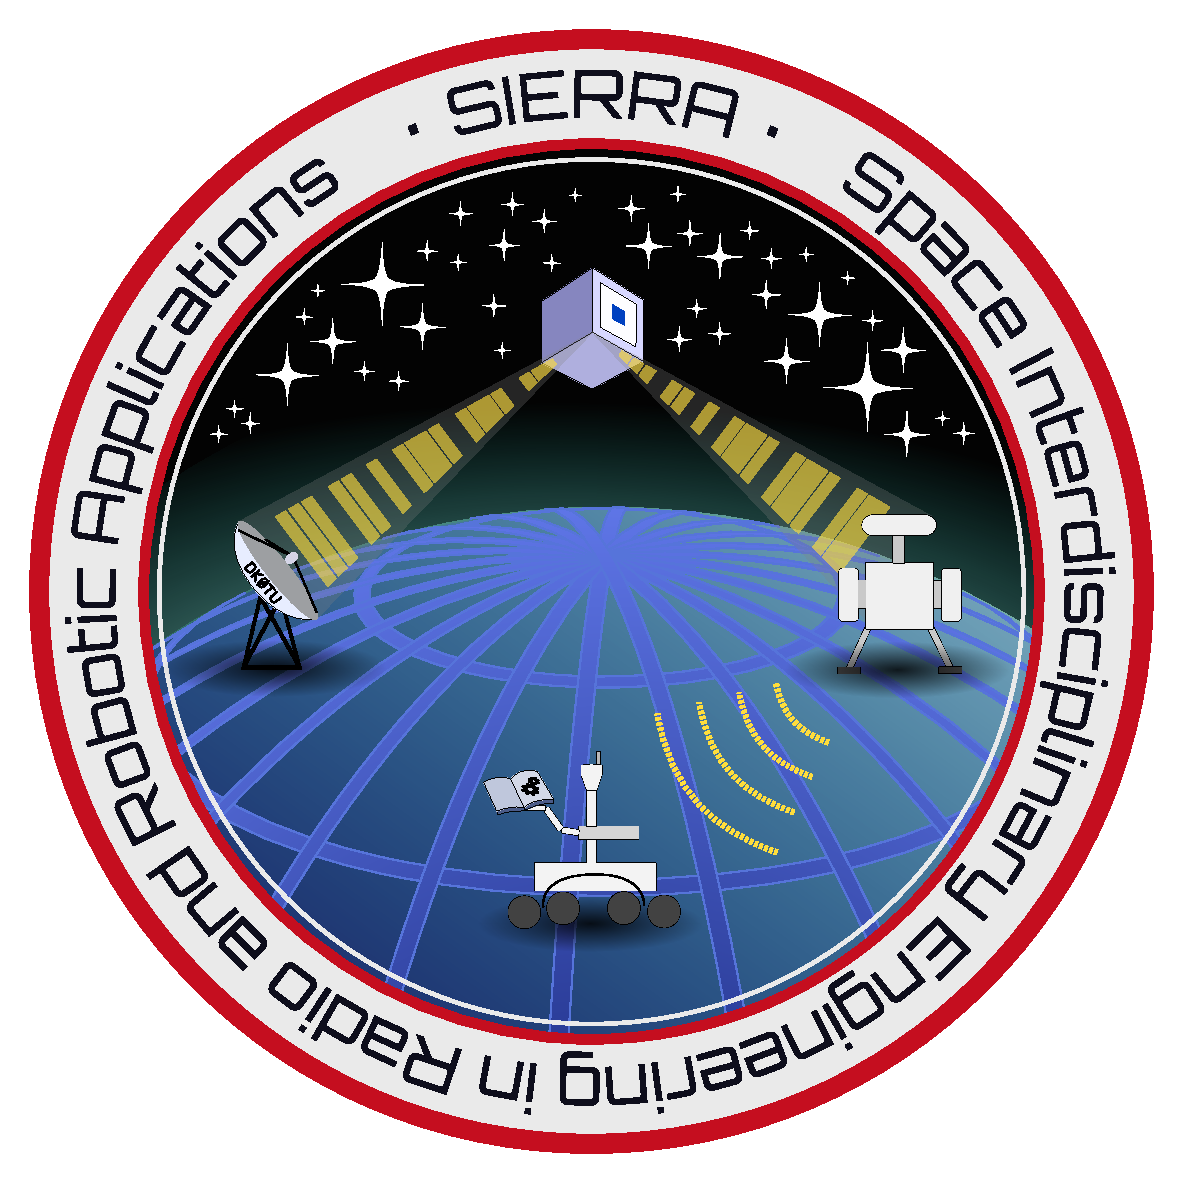
\includegraphics[height = 90mm]{sierra_r4.pdf}
  };
  \end{tikzpicture}
  \begin{center}
    \hspace{0pt}\vfill

    %\large Space Interdisciplinary Engineering in Radio and Robotic Applications \\ \hspace{0pt}

    \huge\textbf{Official Documentation} \\ \vspace{20pt}

    \large{Berlin Experimental and Educational Ground Station}

    \vfill

    \normalfont\normalsize Document: \nr \\
    Version: \ver\\
    Date: \dat

    \vfill

    %
\includegraphics[height=\hh]{../../global_references/tuBerlinLogoRot}
    %
\includegraphics[height=\hh]{../../global_references/tuBerlinLogoSchwarz}

    \normalfont\normalsize \hspace{0pt}\\
    Technische Universit\"at Berlin\\
    Department of Aeronautics and Astronautics\\
    Chair of Space Technology\\
    Office F 6\\
    Marchstra�e 12--14\\
    10587 Berlin

    Tel.: 030 / 314-21305\\
    Fax: 030 / 314-21306
  \end{center}
\end{titlepage}


%%%%%%%%%%%%%%%%%%%%%%%%%%%%%%%%%%%%%%%%%%%%%%%%%%%%%%%%%%%%%%%%%%%%%%%%%%%%%%%

\begin{titlepage}
  \begin{center}
    \textbf{\huge{Technical Note}\\\hspace{0pt}}
    %\textbf{\large{This is an mple headline}\\\hspace{0pt}}
    
    \ \\
    \ \\
    \textbf{Version History\\\hspace{0pt}}
    
    \begin{tabular*}{\textwidth}
      {%
        @{}p{0.1\textwidth}
        p{0.15\textwidth}
        p{0.35\textwidth}
        p{0.3\textwidth}@{}
      }
      \toprule
      Version & Date & Changes & Processor \\
      \midrule
      0.1 & 2021-07-05 & Document creation  & Alexis Cabana-Loriaux \\
      \bottomrule
    \end{tabular*}%
    
    \vfill
    
    \thispagestyle{TUB}
    
    \pagebreak
    
     
    
    
    
    
  \vfill

     \end{center}%
  \thispagestyle{TUB}%
\end{titlepage}

%%%%%%%%%%%%%%%%%%%%%%%%%%%%%%%%%%%%%%%%%%%%%%%%%%%%%%%%%%%%%%%%%%%%%%%%%%%%%%%

	
	\clearpage
	
	%%%% INHALT %%%%
	\pagenumbering{Roman}
	\addcontentsline{toc}{chapter}{Table of Contents}
	\tableofcontents
	\newpage
	\listoffigures
	
	\subpdfbookmark{Contents}{tables}
	\belowpdfbookmark{Contents}{toc}
	
	\clearpage
	\def\thechapter{\arabic{chapter}00}
	\setcounter{chapter}{3}
	\chapter{Portable Rotator Concept}
	\pagenumbering{arabic}
	
	%%%%%%%%%%%%%%%%%%%%%%%%%%%%%%%%%%%%
	% your documentation here
	%%%%%%%%%%%%%%%%%%%%%%%%%%%%%%%%%%%%
	
	\section*{Abstract}
	\addcontentsline{toc}{section}{Abstract}
	
	This report demonstrates an overview of the planning process and work carried out throughout the semester by the team to design and build a new antenna rotator concept.
	
	\section{Introduction}
Various rotators are available and used in controlling the attitude of different types of antennas. For this project the motivation is to develop a new concept to be used with a portable station and able to track satellites, and to achieve this it is designed to move in both azimuth and elevation directions. To meet the requirements, the rotator is characterized by being low cost and based on commercial off-the-shelf parts to compete with available models on the market. \\
The idea is to have a transportable and remotely controllable rotator to test the signal strength of telemetry data that is received in different locations from satellites in a low earth orbits.\\
This concept can be replicated by other interested individuals and is open for improvements. \\
The sections of the report are divided into mechanical and electronic design of the product and covers its calibration and testing plan.

	\section{Project Planning}
	
Initially the system performance requirements were defined. It should be noted however that the team could not manage to meet some of these requirements within the project timeline, specifically OR01, and ER03.
\subsection{System requirements}
\textbf{FR01}: The rotator must be able to move the antenna around the vertical and lateral axis.\\
\textbf{FR02}: The rotator should have a pointing accuracy of $2\degree$.\\
\textbf{FR03}: The rotator should be able to accelerate at $10\degree/s²$ max.\\
\textbf{FR04}: The rotator must have a directional velocity of $5\degree/s$ typical to $20\degree$ max.\\
\textbf{OR01}: The rotator must be able to automatically track satellites.\\
\textbf{ER01}: The rotator must be able to withstand temperatures between $-10\degree C$ and $+40\degree C$.\\
\textbf{ER02}: The rotator must be able to withstand wind loads up to 25 km/s.\\
\textbf{ER03}: The rotator shielding must be able to block rain capacities up to 5 cm/hr.\\
\textbf{LR01}: The rotator must be installable within 10 minutes on site.\\
\textbf{DR01}: The rotator mounting shall be adaptable to standard 35 mm tripod masts.\\
\\
FR: Functional Requirements, OR: Operational Requirements, LR: Logistics Support Requirements, ER: Environmental Requirements, DR: Design Requirement.

\subsection{Work breakdown structure}
The flow of work is subdivided into three main technical branches and the final documentation.
\begin{figure}[H]
	\centering
	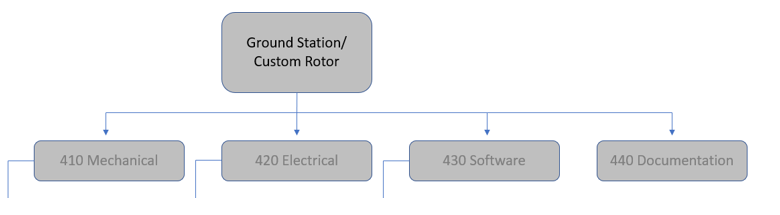
\includegraphics[width=0.8\textwidth]{../art/chart.png}
	\caption{Excerpt from WP-400 work breakdown chart.}
\end{figure}
	
	\section{Project Work}
	
	\subsection{Mechancial}
	\subsubsection{Rotator head}
\subsubsection*{Concept Overview}
The basic concept of the rotation mechanism relies on an assortment of three bevel gears set up in a T-configuration. The central shaft would be mounted vertically to the main mount and the other collinear shafts each attached to an individual JGY 370 12 V DC motor. The action of these motors against the gear assembly would allow for rotation in both the azimuth and elevation directions. This is achieved through attaching an inverted U-shaped aluminum bracket that forms the main fixture structure of the whole rotator. The sides of the bracket are each attached to one of the driven shafts and their relevant motors, while the top face serves as the mounting location of the antenna and printed circuit boards including the Raspberry Pie 4.\\
When the opposing motors rotate in the same direction i.e. both clockwise, the gears are able to transform this into movement in the azimuth direction. This is due to the reaction against the central fixed gear.\\
However, when ordered to rotate in opposing directions this is translated into gears rotating in the same direction against the central gear. This of course will not be physically possible and hence the gear point is fixed, and the rotation motion is transferred to the motors themselves around the axis and by that consequently moving the bracket up or down, changing the elevation sense of the antenna.

\begin{figure}[H]
	\centering
	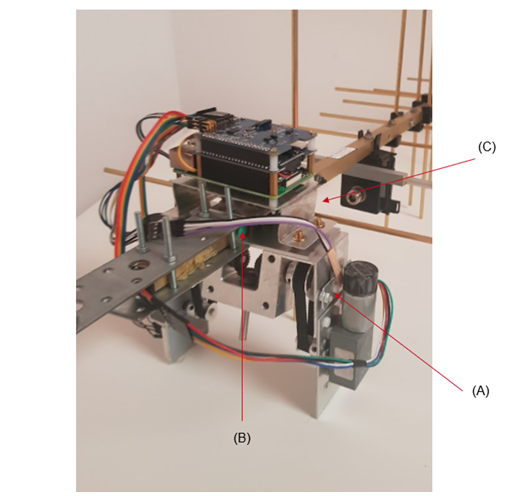
\includegraphics[width=0.8\textwidth]{../art/Pic1Head.png}
	\caption{Rotator Head without shielding.}
\end{figure}

\subsubsection*{Design} 
The initial conditions to be met were the first driving parameters for the design. Namely, the required torque was first investigated. Assuming that this portable rotator would not be tested in storms, the highest of the average of wind speeds in Germany was considered, that being during January, and then rounded to get 19.5 km/h. Since we imagined using a cross Yagi antenna for this application, we took into account one face of the boom and calculated the area to be 0.15 m\^2, the directors being cylindrical and of small diameter were also estimated and found to be of negligible effect if exposed to wind drag. This put together along with the reflector and other parts did not amount to much in relation to torque requirements. The torque required was calculated to be less than 0.25 N however we decided to use this value for safety, and to allow more flexibility for use with other types or shapes of antennas. Separately the average torque of one motor was found to be around 1.3 N/m. While this was sufficient and tested on the first prototype to be adequate for controlling the rotator with a dummy weight, we later decided to double this potential by two, and this was achieved by utilizing a belt and pulley system with a ratio of 2:1.\\
The belts and pulleys in concern are those of GT2 pulleys, and 9mm timing belts. The same class of belts and pulleys used in most commercial 3D printers. This design decision seemed logical for two reasons, one being the need of precise movement and transmission without slippage as is the case for 3D printers, and the other being the affordability and availability characteristics of said parts. A permanent relative position and a constant speed ratio are easy to expect using this product while also being able to handle heavy loads. [1]\\
Constrained by the purchased belt length\footnote{Due to logistics the favored belt length could not be available within time and the design was iterated to fit a new belt.} and the available GT2 pulleys we could finally define the distance between the centers of the horizontal gear and motor shafts. This parameter would also aid in defining the length of the side member of the main bracket to allow for this assembly while taking into account mounting locations of other components of the system. \\
This distance mentioned earlier would be the distance required between the pulleys to fit the belt effectively and ensure efficient functionality. We determined this distance by first investigating the outer diameters of each pulley and then plugging it along with the belt length into this equation:\\
\begin{center}
    $\frac{b+ \sqrt{b^2-32(D-d)^2} }{16}=C$
\end{center}
Where $b=4L-6.28(D+d)$, D: Diameter of large pulley, d: Diameter of small pulley, and L = Length of the belt.\\
Another approach was by using the number of teeth of each pulley after determining the tooth style or pitch which is 2mm for our case.\\
\\
The other main distance to be defined for the bracket was the length. This describes the distance between the inner faces of the opposing sides. Those sides are assigned to support both horizontal axis of the gears. Considering many variables, such as dimensional, geometric, and support characteristics of available pillow block flange bearings, gear shaft length, sheet material thickness, and pulley sizes, the final length was defined at 12.3 cm. However, later this value was changed to 13.5 cm due to changes carried out to meet shortcomings in logistics again. This was still achievable by changing multiple aspects of the design to still be able and accommodate the bearings and shafts as required. 
\\
The final two and not very challenging dimensions to define were the width of the bracket and the mounting location of the driven shafts from the upper face of the bracket.
\\
Further into the build, two 6 mm tubes were threaded to fit into the motor shafts as extensions so we can manage to align the pulleys properly. Bushings were added at the end of each horizontal gear shaft right where they interface with the side bearings. These bushings were also drilled as required to allow the bearing's fasteners to go through them and hold onto the shafts. This is due to having the bearings at 8 mm diameter while the shafts are of a 6 mm diameter. These same bushing also serve to protect the magnets glued at the end of the shafts from getting too close to the metallic balls of the bearing\footnote{This is not a concern anymore, however in a previous method of attachment, for a worst case scenario if the magnet miss-aligns for any reason it would still rotate with the shaft as it doesn't get close enough for it to be pulled to one side alone.}. The latter mentioned magnets are positioned as such to allow reading the position of the shaft by two encoders, each mounted on one side of the bracket. Special mounting plates (A) were designed, cut, and drilled to situate those encoders at the right proximity from the magnets. According to our tests a distance beyond 5 mm was sufficient to lose a proper reading and hence we ultimately managed to install them within a clearance of 1 mm for best reading. Spacers were added between the motors and bracket faces to distance the motor ends from the encoders, while both isolating a chance of interference due to the rotating magnet of the motor's encoders and also allowing easy installation and removal of the encoders in case of inspection or issue without having to uninstall the motors and other components of the assembly first.

\subsubsection*{Material Selection}
The antenna at hand weighs no more than 0.5 kg. When balanced in its mounting location on the bracket, the only load of concern is that applying directly downwards on the bridge. A secondary concern would be the torsional load on the same plate when the rotator moves at its lateral axis. Several design solutions were planned, however using the final procurement, it was found that this issue is easily treated by using an aluminum plate thickness of 3 mm. It must be noted that this was not possible in the initial design because a thickness more than 2 mm for the sides would result in other considerations because we are constrained by certain dimensions of the bearing flanges which would lead to disruption of other parameters as well. However, using the modular approach, we were able to simply use an aluminum plate of a larger thickness for the top section.\\
\\
A FEM analysis shows how the current design handles the load of the antenna.\\
\\
(Include simulation here.) Figure.

\subsubsection*{Antenna Strainer}
The design for the antenna mount varied. Two similar concepts were finally tracked, one would be using a bent aluminum sheet, and another is 3D printed.\\
\\
Note: The metal sheet work required a wait time of two weeks in the workshop due to a busy schedule, and the 3D printed part was never delivered as technical problems with the printer were reported during the job.
\begin{figure}[H]
\centering
\begin{subfigure}{.5\textwidth}
  \centering
  \includegraphics[width=.85\linewidth]{../art/Strain1.png}
  \caption{Machined part.}
  \label{fig:sub1}
\end{subfigure}%
\begin{subfigure}{.5\textwidth}
  \centering
  \includegraphics[width=.85\linewidth]{../art/Strain2.png}
  \caption{3D printed part.}
  \label{fig:sub2}
\end{subfigure}
\caption{This figure shows two of the final antenna holders.}
\label{fig:test}
\end{figure}
On the final presentation the antenna was fixed using a sandwich of aluminum plates, constrained by 3 bolts on each side, and wrapped in a rubber material (B) as an interface between the antenna boom and the bolts and plates to increase traction considerably and avoid any chance of slippage during operation (Figure 2).

\subsubsection*{PCB Mounting}
A custom-made bridge (C) was drawn and fabricated to mount the PCB sandwich (Figure 2).

	\subsubsection{Weather shielding}
The custom rotator is designed to operate in outdoor environment for long duration. To avoid damage from sun light exposure and humidity, a dedicated shielding is designed for mechanical and electronics parts. The architecture of shielding is based on consideration that shielding should not hinder the mechanical movements of any part. 
\subsubsection*{Weather shielding design methodology}
The design of shielding is optimised to provide protection to the critical parts. Materials, manufacturing process and parts are from off shelf technologies and easy to manufacture. Manufacturing materials are aluminium sheet and 3D printed abs plastic. Following figure shows various components of shielding marked in green and white colour.     
\begin{figure}[H]
	\centering
	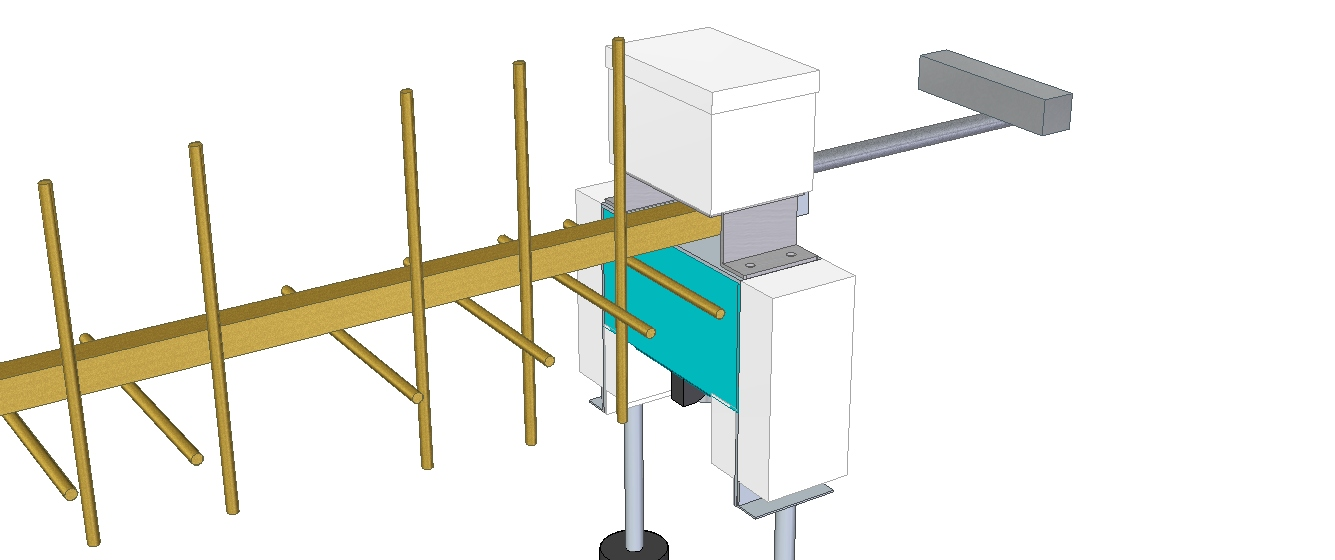
\includegraphics[width=\linewidth]{../art/overing.jpg}
	\caption{Rotator with Shielding}
\end{figure}

The differential shielding (green color) is responsible to provide free movement to the rotator. The design is inspired from the military vehicle design. In this approach, a grove is provided for movement of shaft and this whole structure is covered with a flexible sheet (black in colour) to provide movement capability and seal. 

\subsubsection*{Belt covering}
Belt covering is provided by 3D printed abs plastic structure and mounted by nuts and bolts on main frame. It provides easy access for repair and routine checks. Following image shows the design and the way it is going to cover the belt and pulley. The remaining top of the belt will be covered in differential shielding.     
\begin{figure}[H]
	\centering
	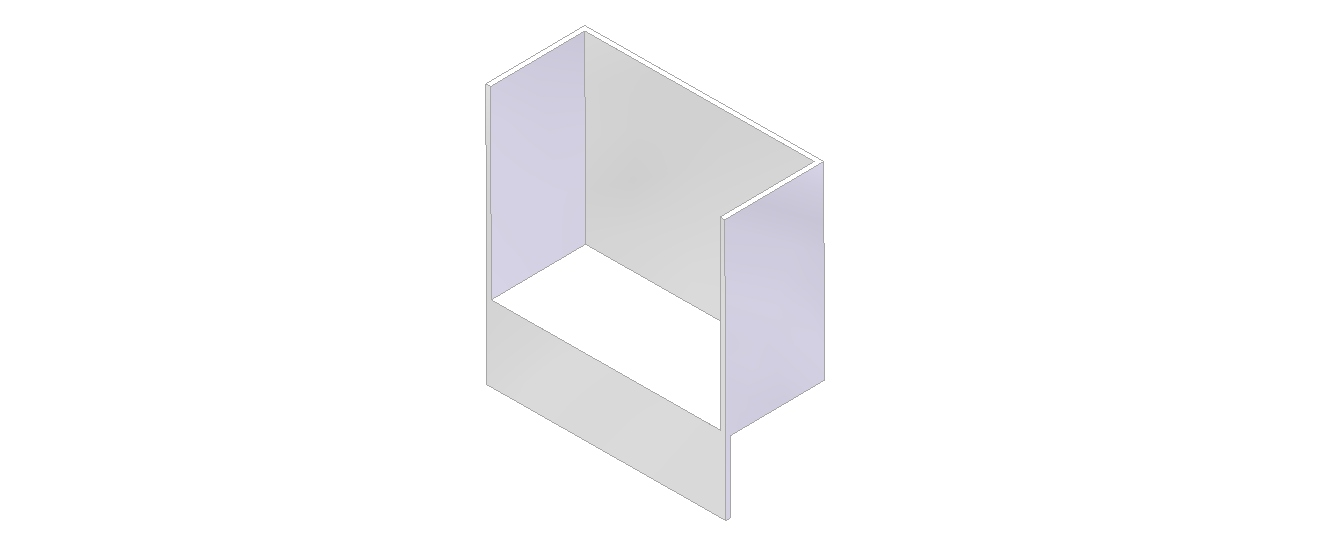
\includegraphics[width=0.7\linewidth]{../art/belt cover.jpg}
	\caption{Belt Covering}
\end{figure}

\subsubsection*{Motor covering}
Motor covering is provided by 3D printed abs plastic structure and mounted by nuts and bolts on main frame. It provides easy access for repair and routine checks. Following image shows the design and the way it is going to cover motor.     
\begin{figure}[H]
	\centering
	
\includegraphics[width=0.8\linewidth]{../art/motor cover.jpg}
	\caption{Motor Covering}
\end{figure}

\subsubsection*{Electronics Covering}
Electronics box is designed by using 3D printed abs plastic structure and mounted by nuts and bolts on main frame. It provides easy access for repair and routine checks. It is simple cuboid box with top cover lid. It is designed to provide required volume for controllers, receiver and wiring.    
\begin{figure}[H]
	\centering
	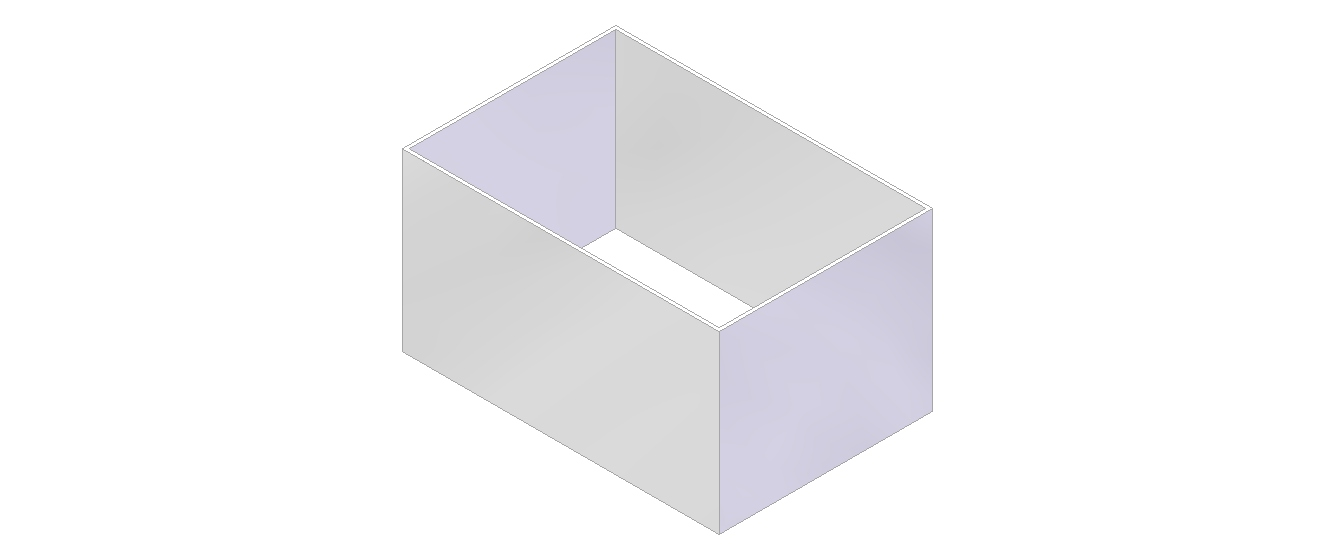
\includegraphics[width=0.7\linewidth]{../art/elec.jpg}
	\caption{Electronics Covering}
\end{figure}


    \subsubsection{Mount interface}
Rotator is designed to be mounted on tripod and can be deployed outdoors. To fulfil this requirement a standard mount is designed which can provide mechanical joint between differential shaft of rotator and tripod rod as shown in following figure 400.8.  
\begin{figure}[H]
	\centering
	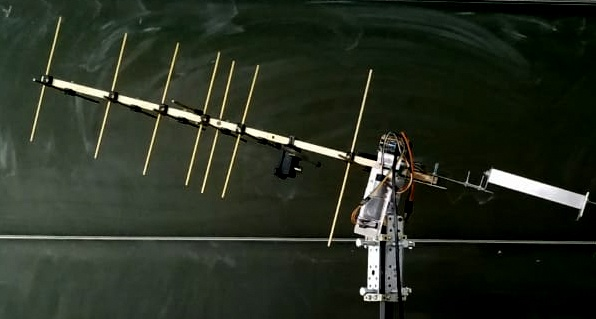
\includegraphics[width=\linewidth]{../art/real image.jpeg}
	\caption{Mount Prototype}
\end{figure}

\subsubsection*{Mount interface design methodology}
Design of mount is inspired from lathe chuck which has mechanism to hold any work-piece. In this design similar capability is achieved by providing 8 nut bolts which can hold tripod of 10 mm to 40 mm diameter. Further this design has capability to compensate levelling of rotator with respect to horizon by 10 deg. on each side. Following figure shows mount and it’s connection differential gear.   

\begin{figure}[H]
	\centering
	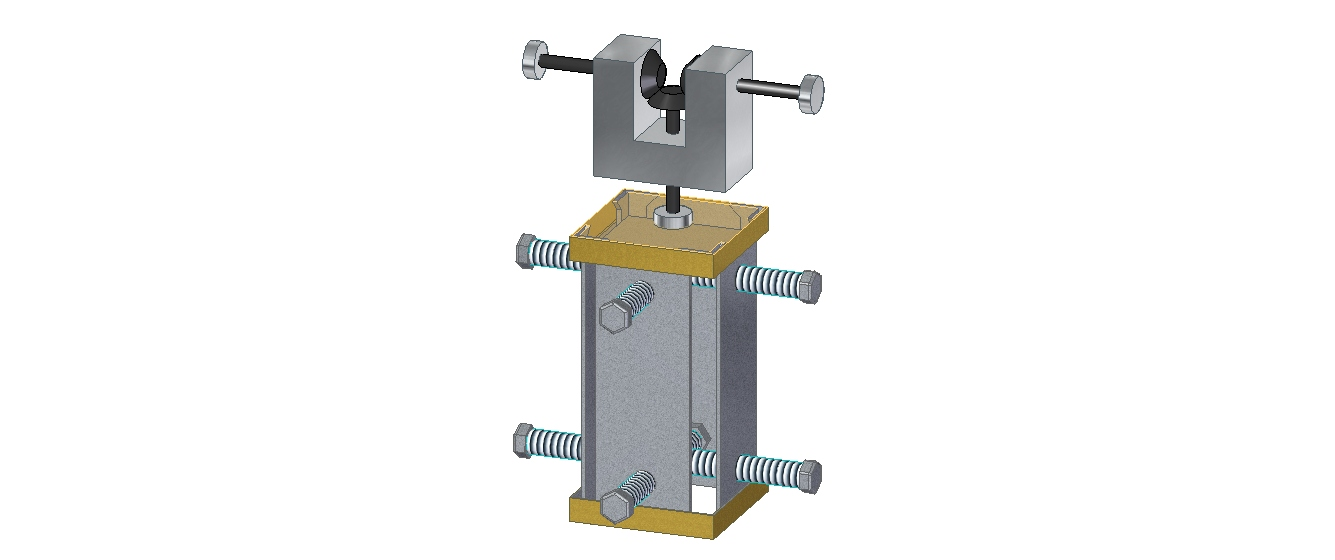
\includegraphics[width=0.9\linewidth]{../art/m.jpg}
	\caption{Mount image CAD}
\end{figure}

\subsubsection*{Scope of improvements}
Other mounting options can be explored to reduce the cost and complexity of the design. These improvement can be implemented by using off the shelf technologies. One of the option is usage of sound box adaptor for mount as shown in figure 400.10.     

\begin{figure}[H]
	\centering
	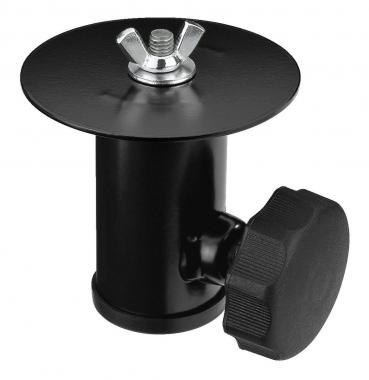
\includegraphics[width=0.2\linewidth]{../art/buy mount.jpg}
	\caption{Example of off shelf technology}
\end{figure}	
    \subsubsection{Counter weights}
\subsubsection*{Arm weight balancing}
After deciding on the section of the boom that would be fixed to the rotator, we proceeded to determine the required force and its location to neutralize the weight acting on the antenna arm for this pivot point. We found the center of gravity of the antenna and then commenced moving it backwards until it sits at the center of the upper plate where it is mounted. A mass of 0.8 kg was calculated to be required at 13.5 cm from the center (from center to center). This value varies slightly depending on the shape of the weight attached. Conveniently, we found some microphone boom weights with the same value and that also attach to the same diameter of the boom we have. However sometimes an adapter might be required, and this would have slight implications on the position of the counterweight as we take into account the additional mass in that location. Figures 400.11 and 400.12 show the counter weight options. 
\begin{figure}[H]
	\centering
	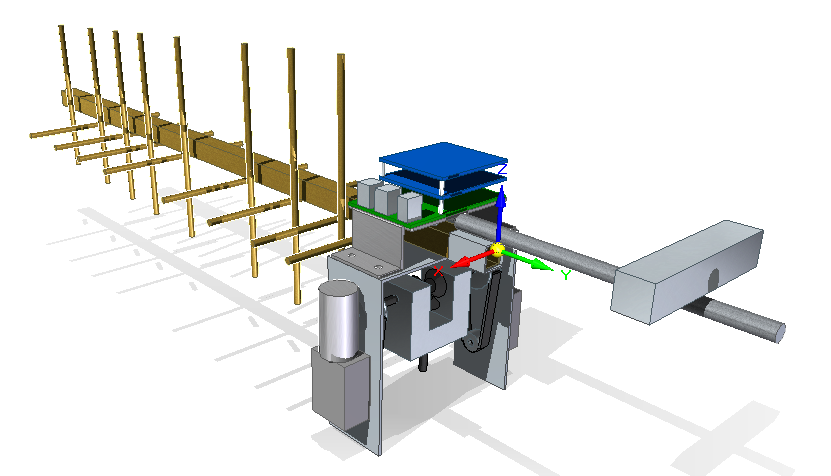
\includegraphics[width=0.5\textwidth]{../art/isoback.png}
	\caption{Arm weight balancing}
\end{figure}

\begin{figure}[H]
	\centering
	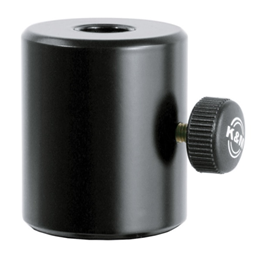
\includegraphics[width=0.2\textwidth]{../art/weight1.png}
	\caption{Commercial 0.8 kg counter weight. [2]}
\end{figure}





\subsubsection*{Pitch mass shift compensation} 
Pitch mass shift counter weights are used to balance the centre of gravity in vertical axis. The final target is to balance centre of gravity at rotational axis of the rotator. This will put negligible load on motors and motors have to overcome just inertia. The considered rotator design requires balancing of centre of gravity in both horizontal and vertical axis.  To compensate real case variations, dead weights are mounted on COTS threaded rods. This helps the user to balance the centre of gravity with extreme accuracy. Figure 400.13 shows the pitch mass weights. 


\begin{figure}[H]
	\centering
	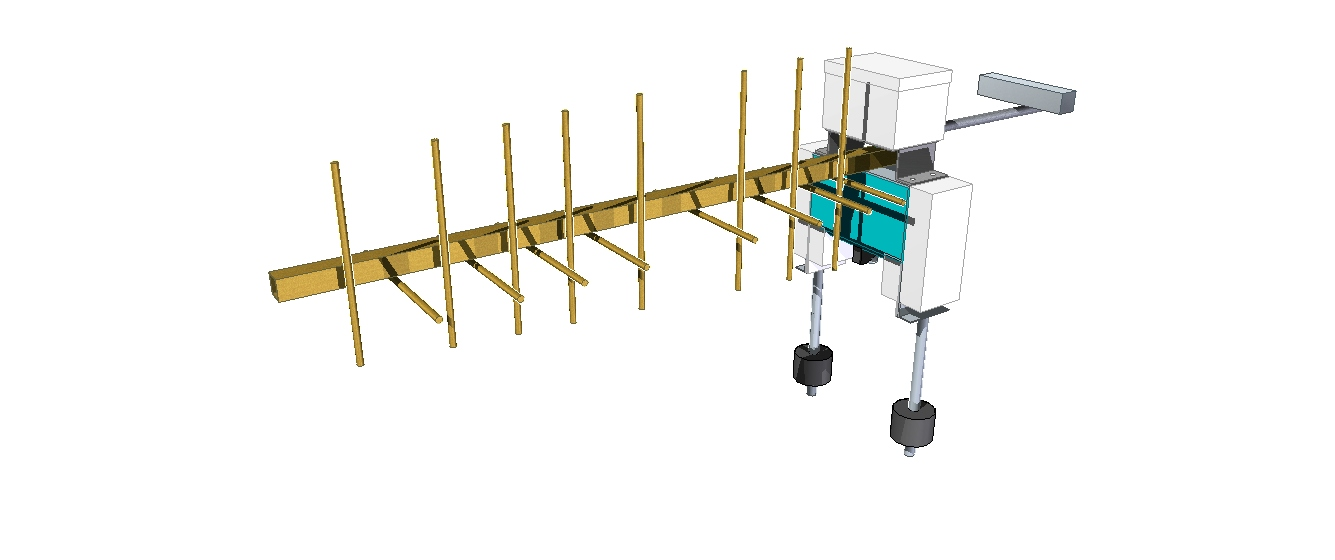
\includegraphics[width=1\textwidth]{../art/isoshield.jpg}
	\caption{Pitch mass weights}
\end{figure}

	
	
	\subsection{Electronics}

Electronics of this project

\begin{figure}[h]
	\centering
	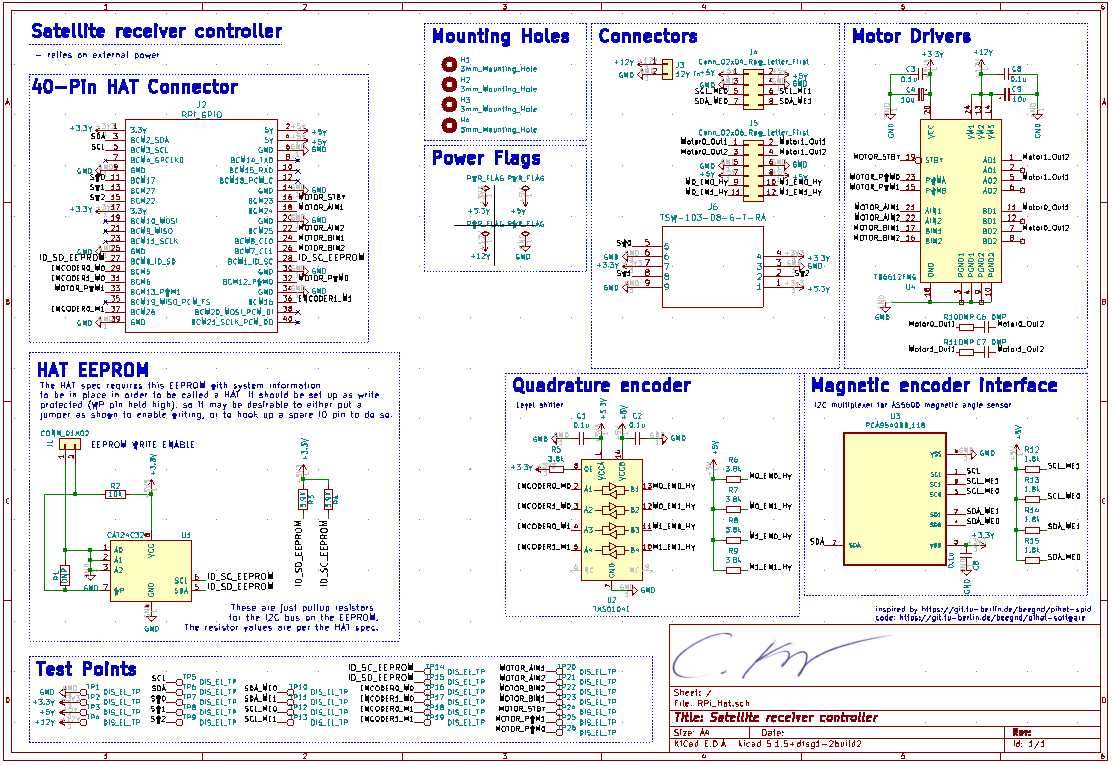
\includegraphics[width=\linewidth]{../art/pcbSchematic.png}
	\caption{Schematic of Raspberry Pi hat}
\end{figure}


\begin{figure}[h]
	\centering
	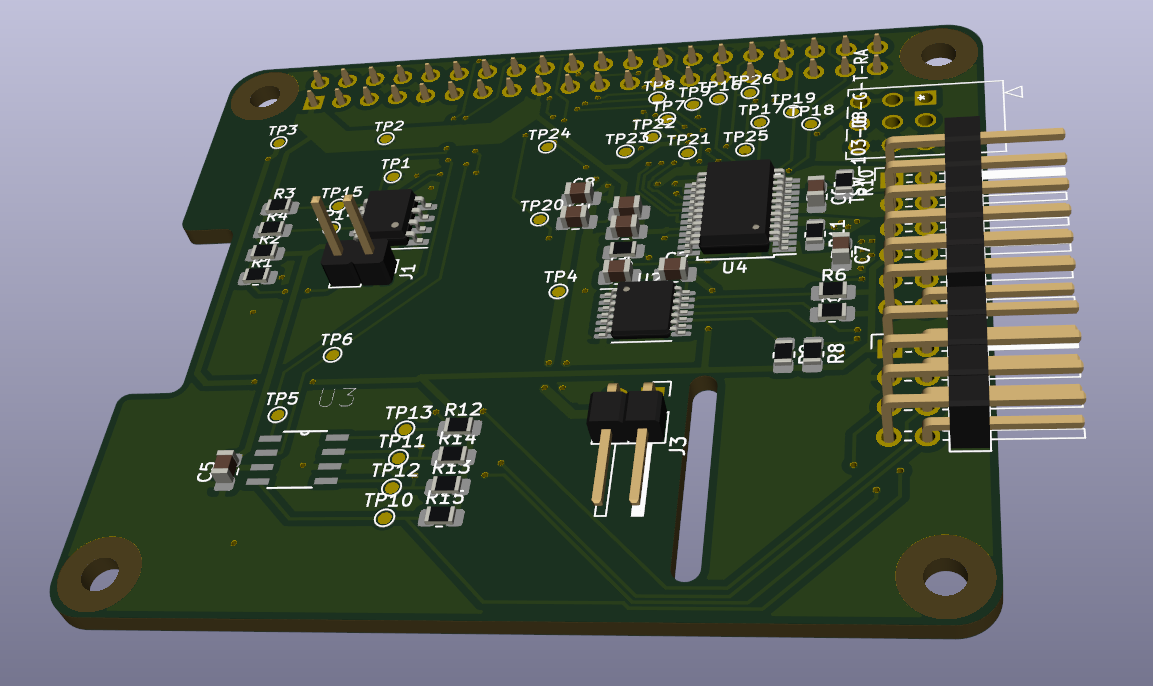
\includegraphics[width=\linewidth]{../art/PCB.png}
	\caption{PCB of Raspberry Pi hat}
\end{figure}

	\subsection{Code}

\subsubsection{Quick start}
The code is executed by the Raspberry Pi. The python script needs to be started manually. For example, you could connect to the pi via ssh on the command line. If you know the IP address of the Raspberry Pi, you can log in via (default password is 'raspberry'): 

\begin{verbatim}
ssh pi@ipAdress
\end{verbatim}

If you don't know your Raspberry Pi's IP address, you can connect the raspberry's Ethernet cable directly to your pc. See this  \href{https://www.circuitbasics.com/how-to-connect-to-a-raspberry-pi-directly-with-an-ethernet-cable/}{Guide} or this 
\href{https://stackoverflow.com/questions/16040128/hook-up-raspberry-pi-via-ethernet-to-laptop-without-router}{Guide}. If you set up the Raspberry Pi for the first time, note the src/README.md in the \href{https://github.com/EagleEyeElite/satelliteReceiver}{git repository}. Once you are logged in, start the rotctl service:

\begin{verbatim}
source ./venv/bin/activate
cd satelliteReceiver/src/
./main.py     # start controller
\end{verbatim}

Connect to the started rotctl service from your pc:
\begin{verbatim} 
rotctl -m 2 -r 10.42.0.101:4533
\end{verbatim}


\subsubsection{Code structure}

The code implements the rotctl server. It's multithreaded to serve the clients requests and oversee the rotator simultaneously. The rotator uses two magnetic encoders, connected to the differential, to gain absolute position (even after power cut off). The motor's encoder are used to monitor the motor speed. Additionally, the rotor can observe three safety switches to cut off the motors to prevent the rotator damaging itself.
The code structure represents the structure of the rotator and the electronics. All IC's like the h-bridge, the i2c multiplexer etc. have their own driver modules. The rotator itself and the two shafts connected to the differential are also represented as objects. Note \ref{Code_structure} to see the full code structure:


\begin{figure}[H]
	\centering
	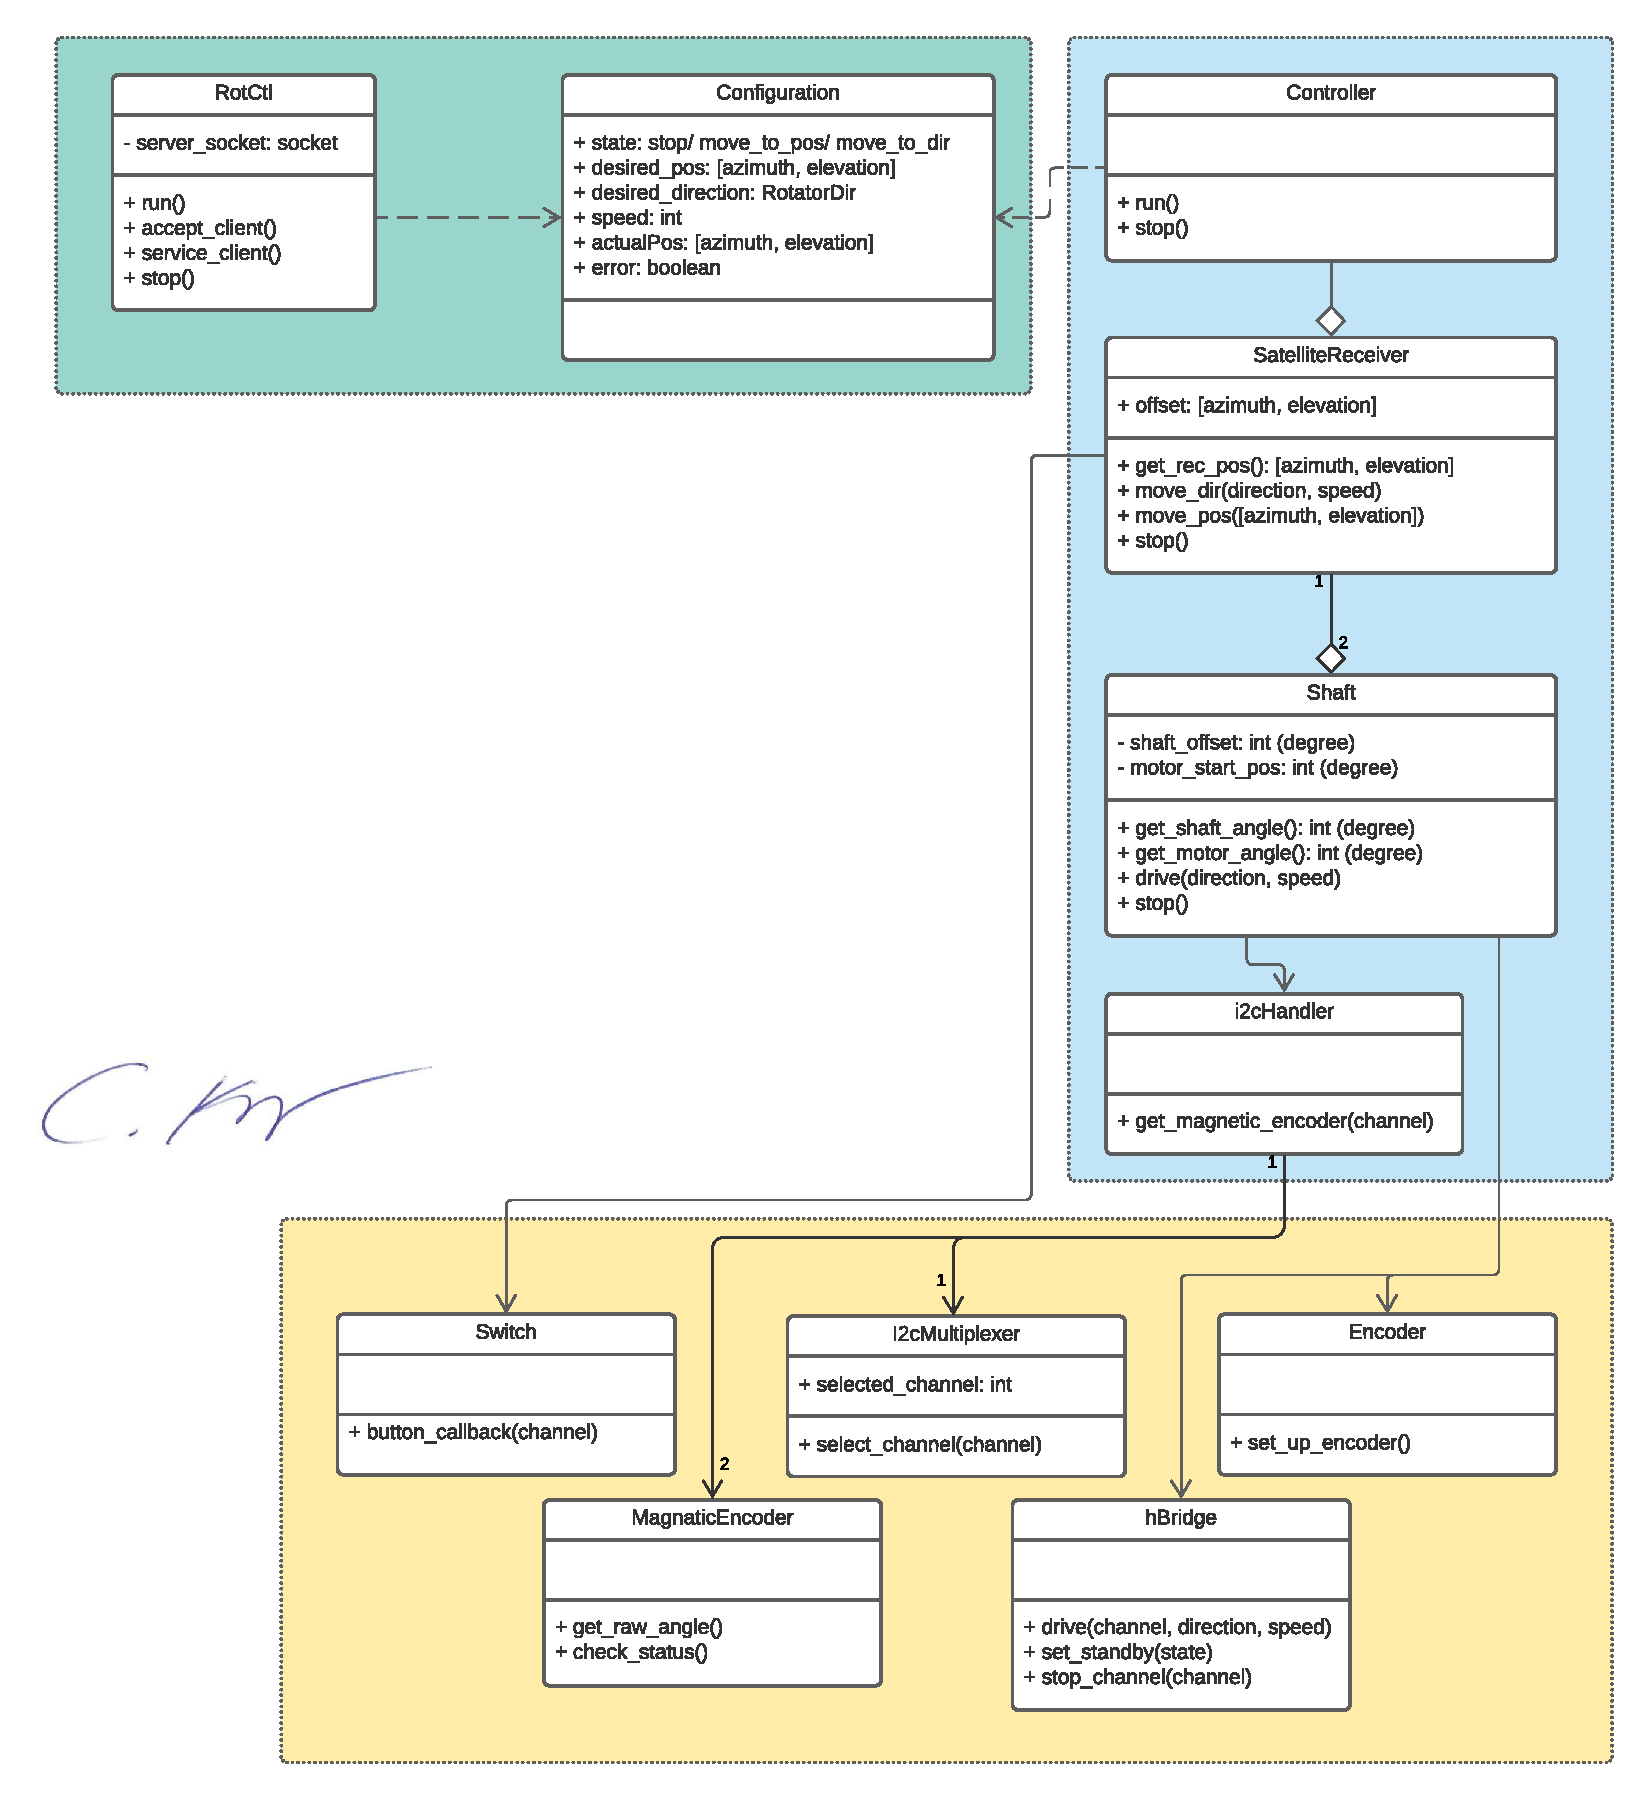
\includegraphics[scale=0.5]{../art/SatelliteReceiver.pdf}
	\caption{Code structure}
	\label{Code_structure}
\end{figure}

Once the python script is started, two independent threads are started. One thread handles all communication to different clients, and the other thread handles the movement of the controller. They interact through a configuration object. The rotctl sets a desired position, direction or a stop signal. It also reads out the current actual position of the rotator. The Controller on the other hand read out the desired position, direction and the stop signal and sets the actual position.

This separation allows the rotctl server to be non-blocking.

If the client requests position A and then quickly request position B, the rotator doesn't need to wait until it moved to position A to then move the position B. With this separation it can simply discard the old request and move to the new request immediately.

All values in the configuration object are always updated by only one thread. The values are also not used for further computation. Even though racing condition can occur, the code is still thread safe.

\begin{figure}[H]
	\centering
	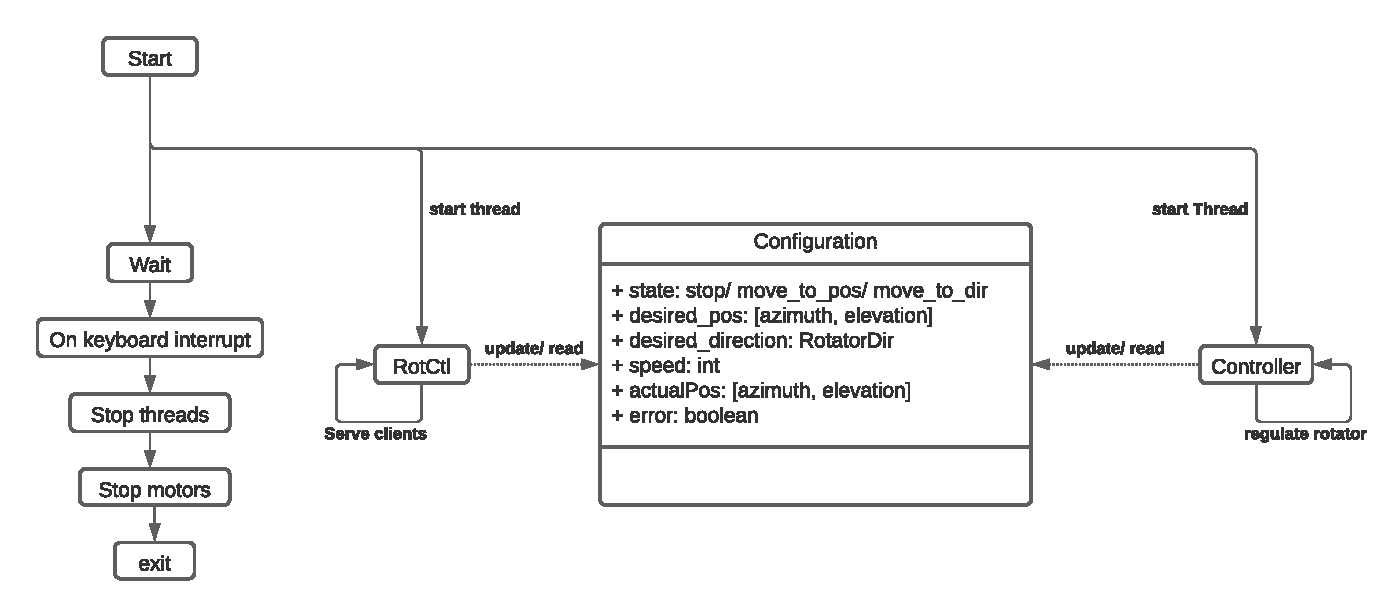
\includegraphics[width=\linewidth]{../art/Code flow chart.pdf}
	\caption{Raspberry Pi HAT flow diagram}
\end{figure}

\subsubsection{Possible improvements}
The time constrains didn't allow to make any real use of the EEPROM on the pi hat. With more time, it would be possible to save a configuration on that EEPROM, to set up pi the pi automatically. The I2C bus, for example, could be enabled, as soon as the board is plugged in.

In a demonstration video, we showed the movement of the rotator. The readings of all sensors work well. Unfortunately, more testing is required on the position calculation. As of now, we still assume some bugs in the algorithm to get the current position. The safety switches are included in the code, but not yet on the actual rotator. It's effortless to stop the rotator at any given time per command over rotctl or over the ssh connection. Playing around with it doesn't introduce a huge risk. But we don't recommend putting it up somewhere and to expect, that it doesn't break itself eventually.
	
	
	\section{Conclusion}
	We enjoyed working on the project and learned a lot. The rotator is great to play around and see it in action. It's not yet in a state, where you can put it anywhere and expect it to work perfectly. If you just want to have something working, that you don't have to worry about and fix from time to time, we recommend using an off the shelf rotator.
	
	\chapter{Appendix}
	\section{PCB schematic and manufacturing process}

\begin{figure}[H]
	\centering
	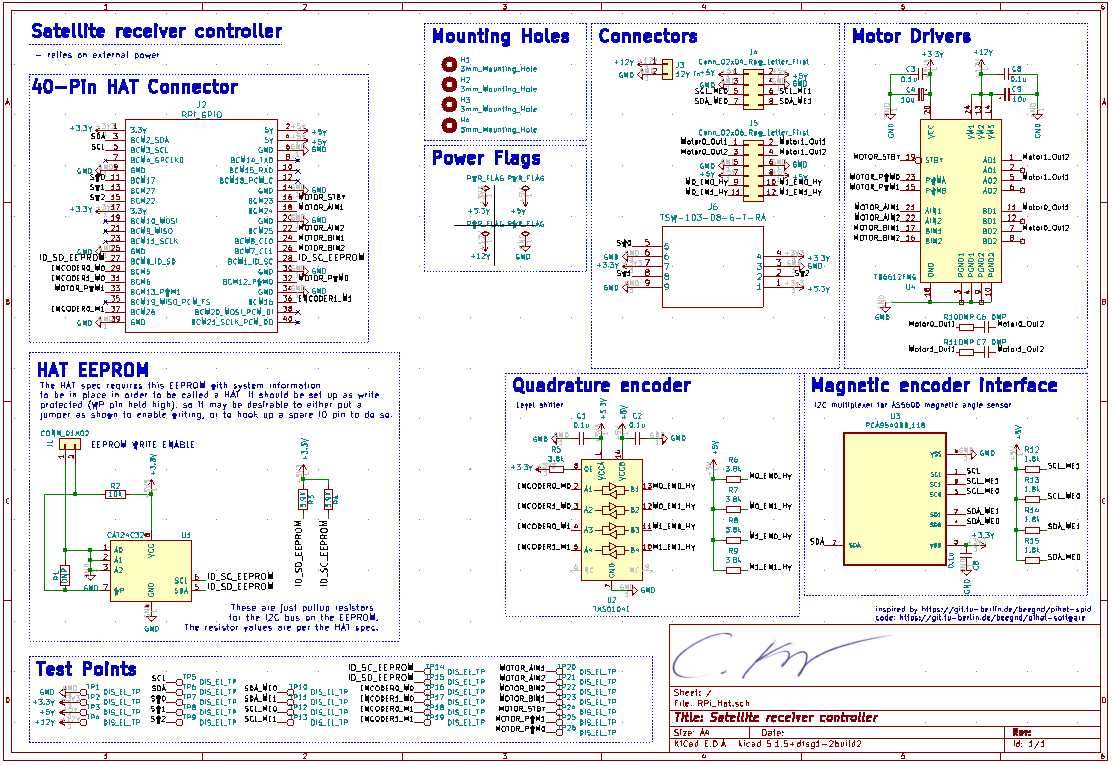
\includegraphics[width=\linewidth]{../art/pcbSchematic.png}
	\caption{Schematic of Raspberry Pi hat}
\end{figure}

\begin{figure}[H]
	\centering
	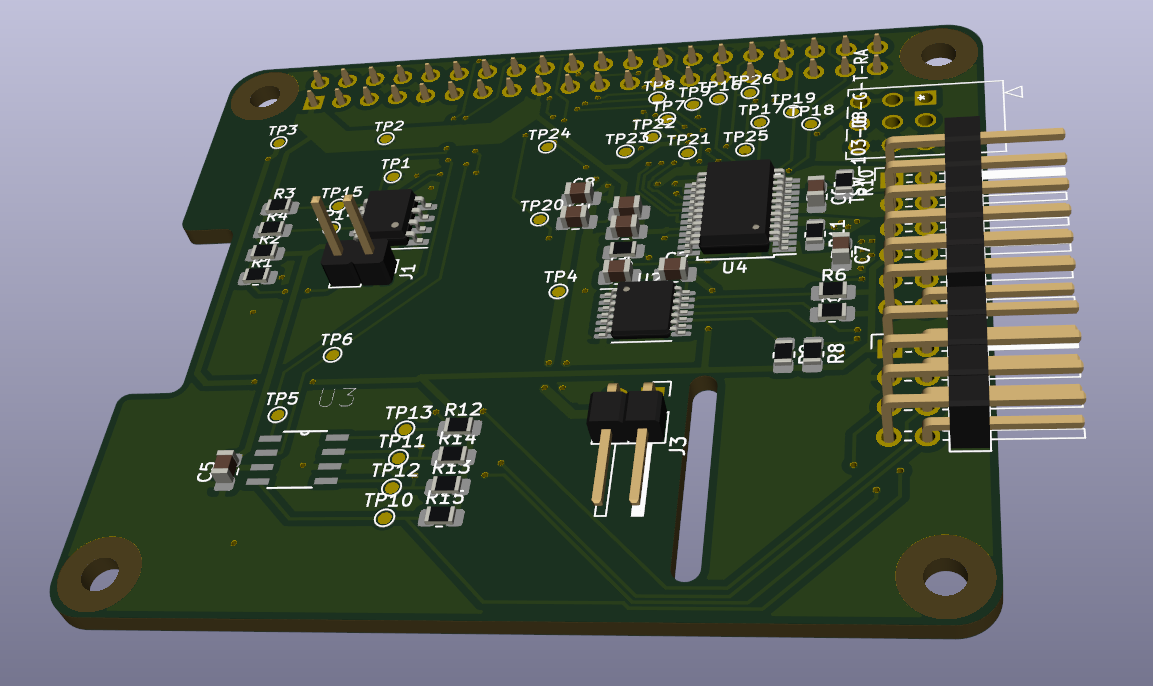
\includegraphics[scale=0.3]{../art/PCB.png}
	\caption{PCB of Raspberry Pi hat}
\end{figure}


\begin{figure}[H]
	\centering
	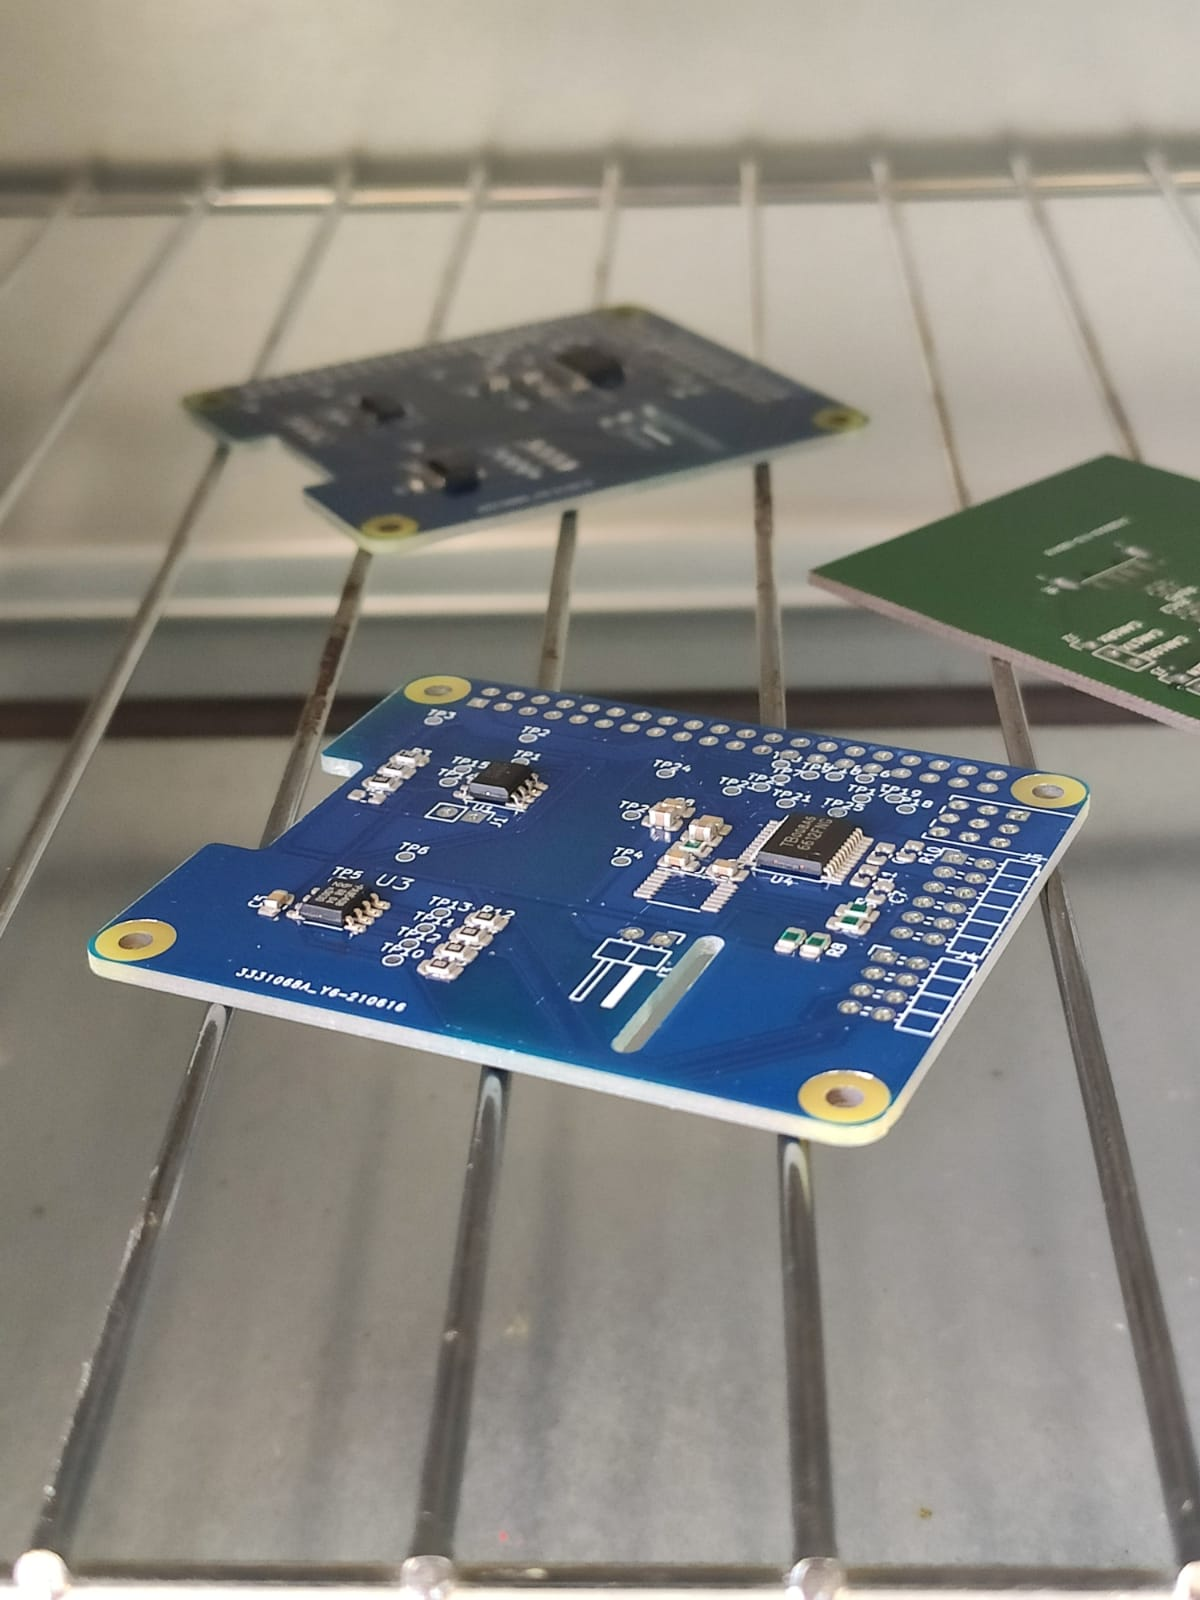
\includegraphics[scale=0.2]{../art/pcb Manufactureing.jpeg}
	\caption{Raspberry Pi hat manufacturing in the reflow oven}
\end{figure}
	\newpage
	
\bibliographystyle{alpha}
\bibliography{sample}
\vspace{0.5cm}

[1] https://www.sdp-si.com/D265/PDF/D265T003.pdf

[2] https://www.k-m.de/en/kmPdf/datasheet/ordernumber/21105-000-55



\end{document}
